\documentclass[12pt,english, journal=jpr, layout=twocolumn]{article}
\usepackage{amsmath,mathtools,amssymb,mathrsfs,dsfont,amsthm}
\usepackage[margin=1in]{geometry}
\usepackage{algpseudocode}
\usepackage{algorithm}
\usepackage[T1]{fontenc}
\usepackage{babel}
\usepackage{graphicx}
\usepackage{float}
\usepackage{color}
\graphicspath{ {figures/} }
\usepackage[colorlinks]{hyperref}
\hypersetup{citecolor=blue}
\usepackage{enumitem}
\usepackage{authblk}
\usepackage{pifont}
\usepackage{lineno}
\usepackage[normalem]{ulem}
\usepackage[export]{adjustbox}
\usepackage{ccaption}
\usepackage{achemso}
\linespread{1.1}

\renewcommand\Affilfont{\itshape\scriptsize}
\renewcommand\Authfont{\small}
\newcommand{\xmark}{\ding{55}}
%opening
\title{Supplement: Challenges and opportunities for Bayesian statistics in proteomics}
\author[1]{Oliver M. Crook \thanks{\url{oliver.crook@stats.ox.ac.uk}}~}
\author[2]{Chun-wa Chung}
\author[1]{Charlotte M. Deane}


\begin{document}
	
\section{Representing uncertainty in common mass-spectrometry quantities}
One quantity that we frequently interested in mass-spectrometry is the sequence of a peptide. There is some uncertainty in a peptide sequence given the relevant spectra. If we quantified the probability in this sequence, we could plot the probability that one amino acid proceeds another as a heatmap, example below:

\begin{figure}[H]
	\centering
	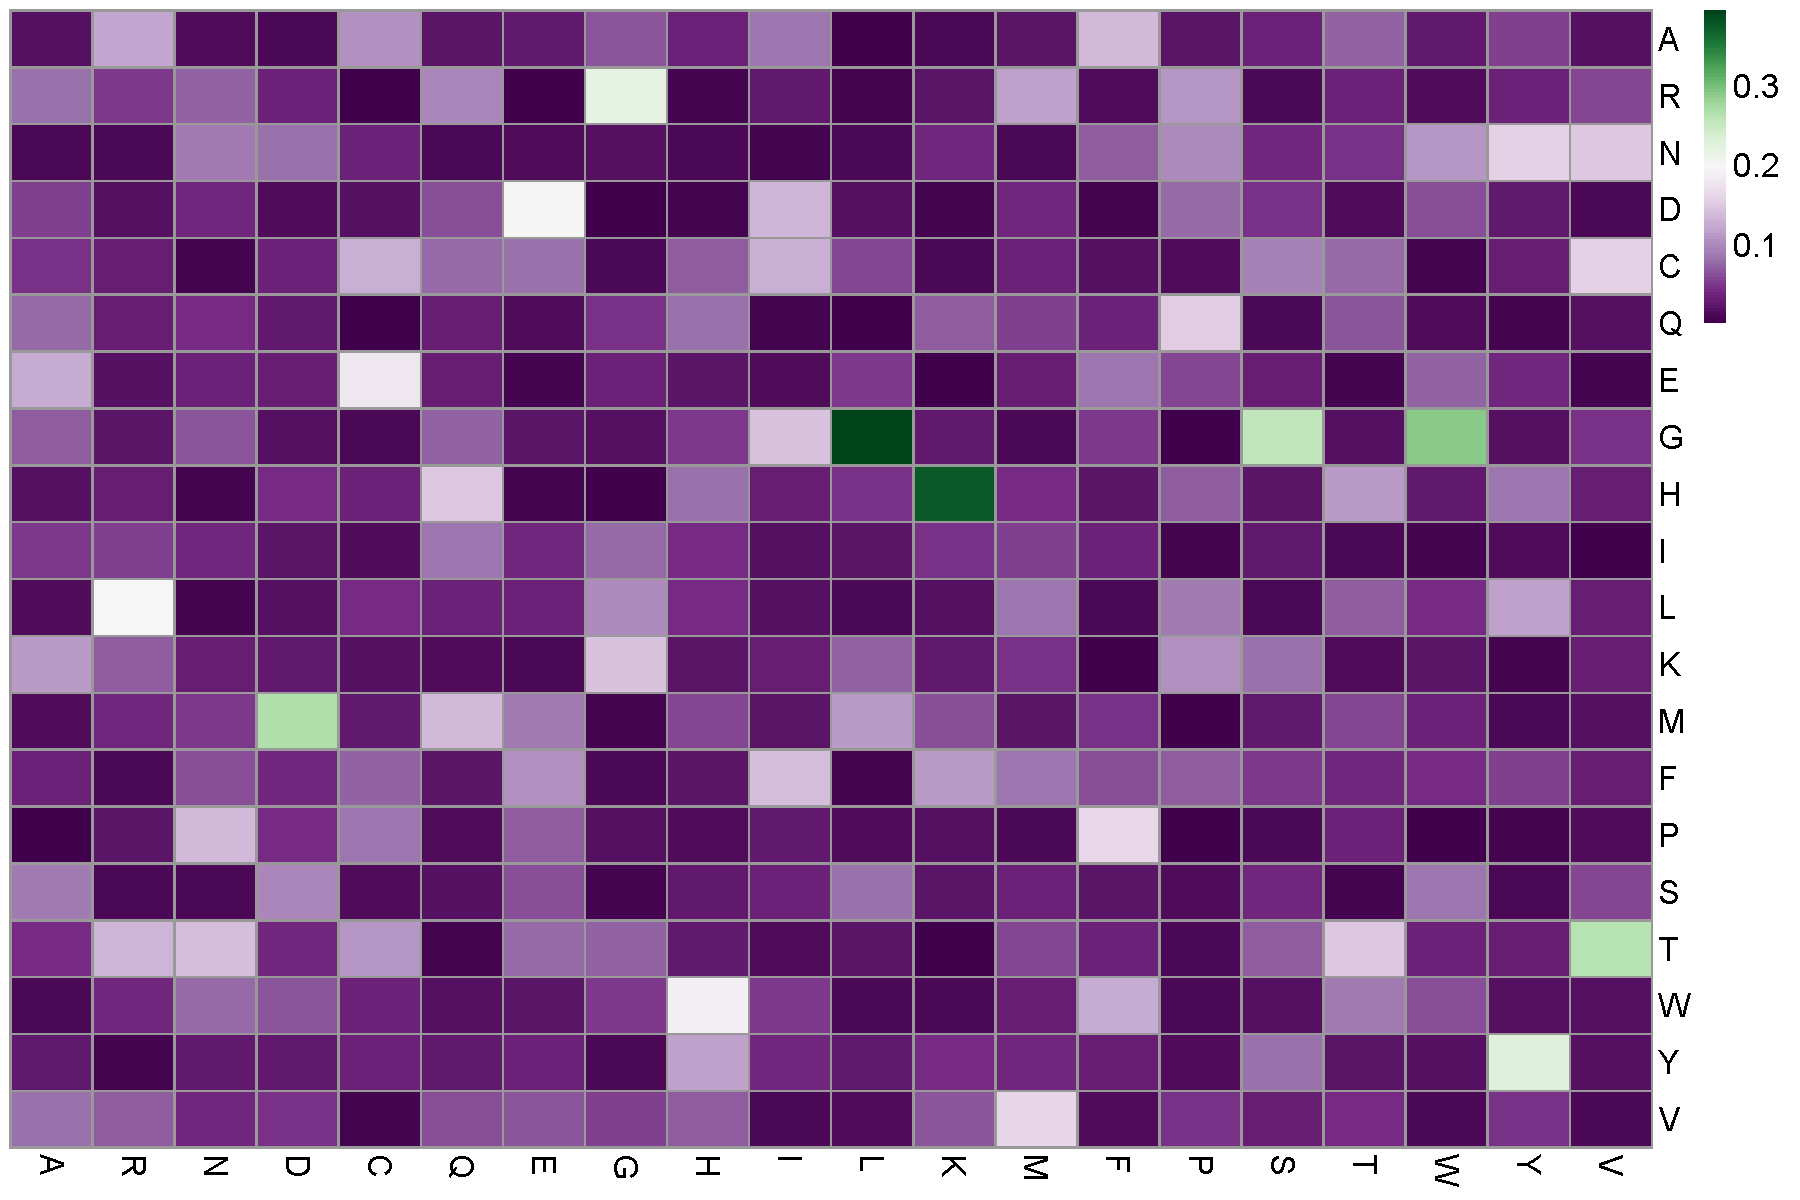
\includegraphics[width =1\textwidth]{probabilityaminoacids.pdf}
	\caption{\textbf{Heatmap of amino-acid probabilities.} A heatmap where the the $(i,j)^{th}$ entry represents the probability that amino acid $i$ is followed by amino acid $j$}.
	\label{figure::figure1aa}
\end{figure}

Another quantity is the uncertainty in a spectra. The following are $9$ MS1 spectra which are all compatible with peptide PARRDAARA with total intensity 1000.
	
\begin{figure}[H]
	\centering
	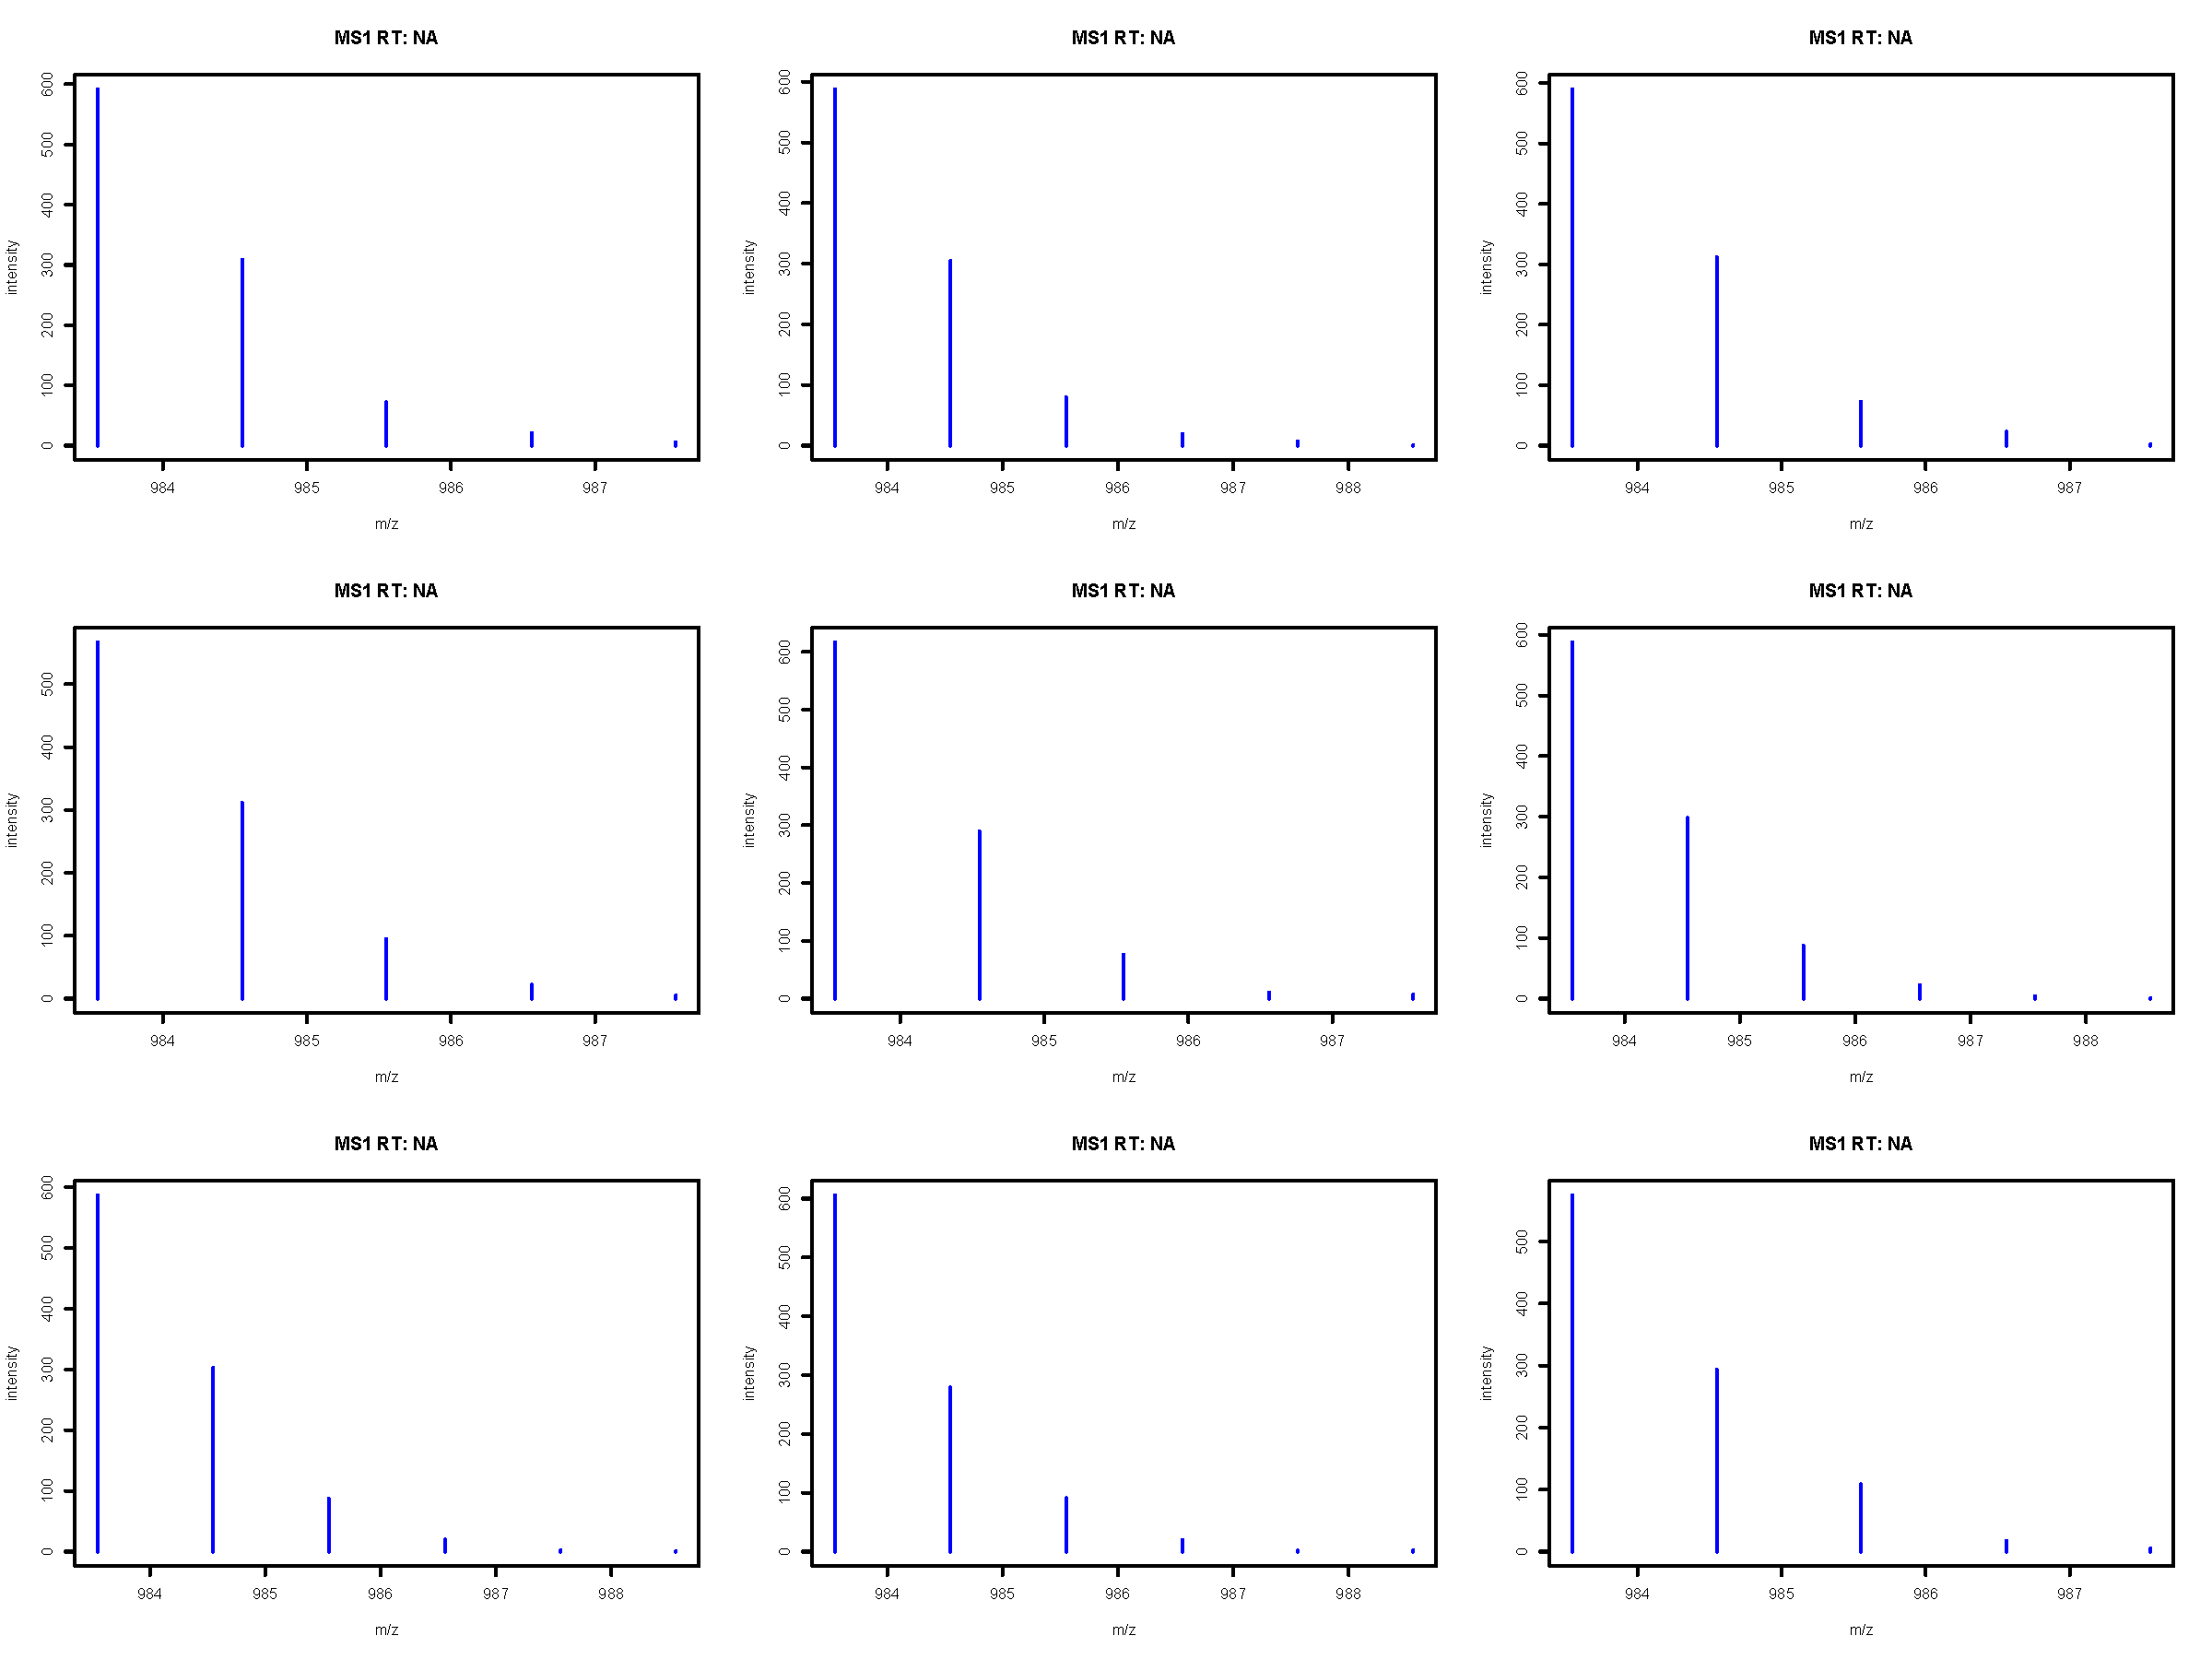
\includegraphics[width =1\textwidth]{aaMS1example.pdf}
	\caption{\textbf{Spectra of PARRDAARA.} Spectra diagrams showing spectra compatible with the MS1 spectra of PARRDAARA}.
	\label{figure::figure2spectraexample}
\end{figure}

It is infeasible to plot the 1000's of spectra that are compatible with MS1 spectra of an amino-acid sequence. Hence, we can use a contour plot which capture the local density of the spectra locations and heights. A typical spectra is overlaid for reference in white.

 \begin{figure}[H]
 	\centering
 	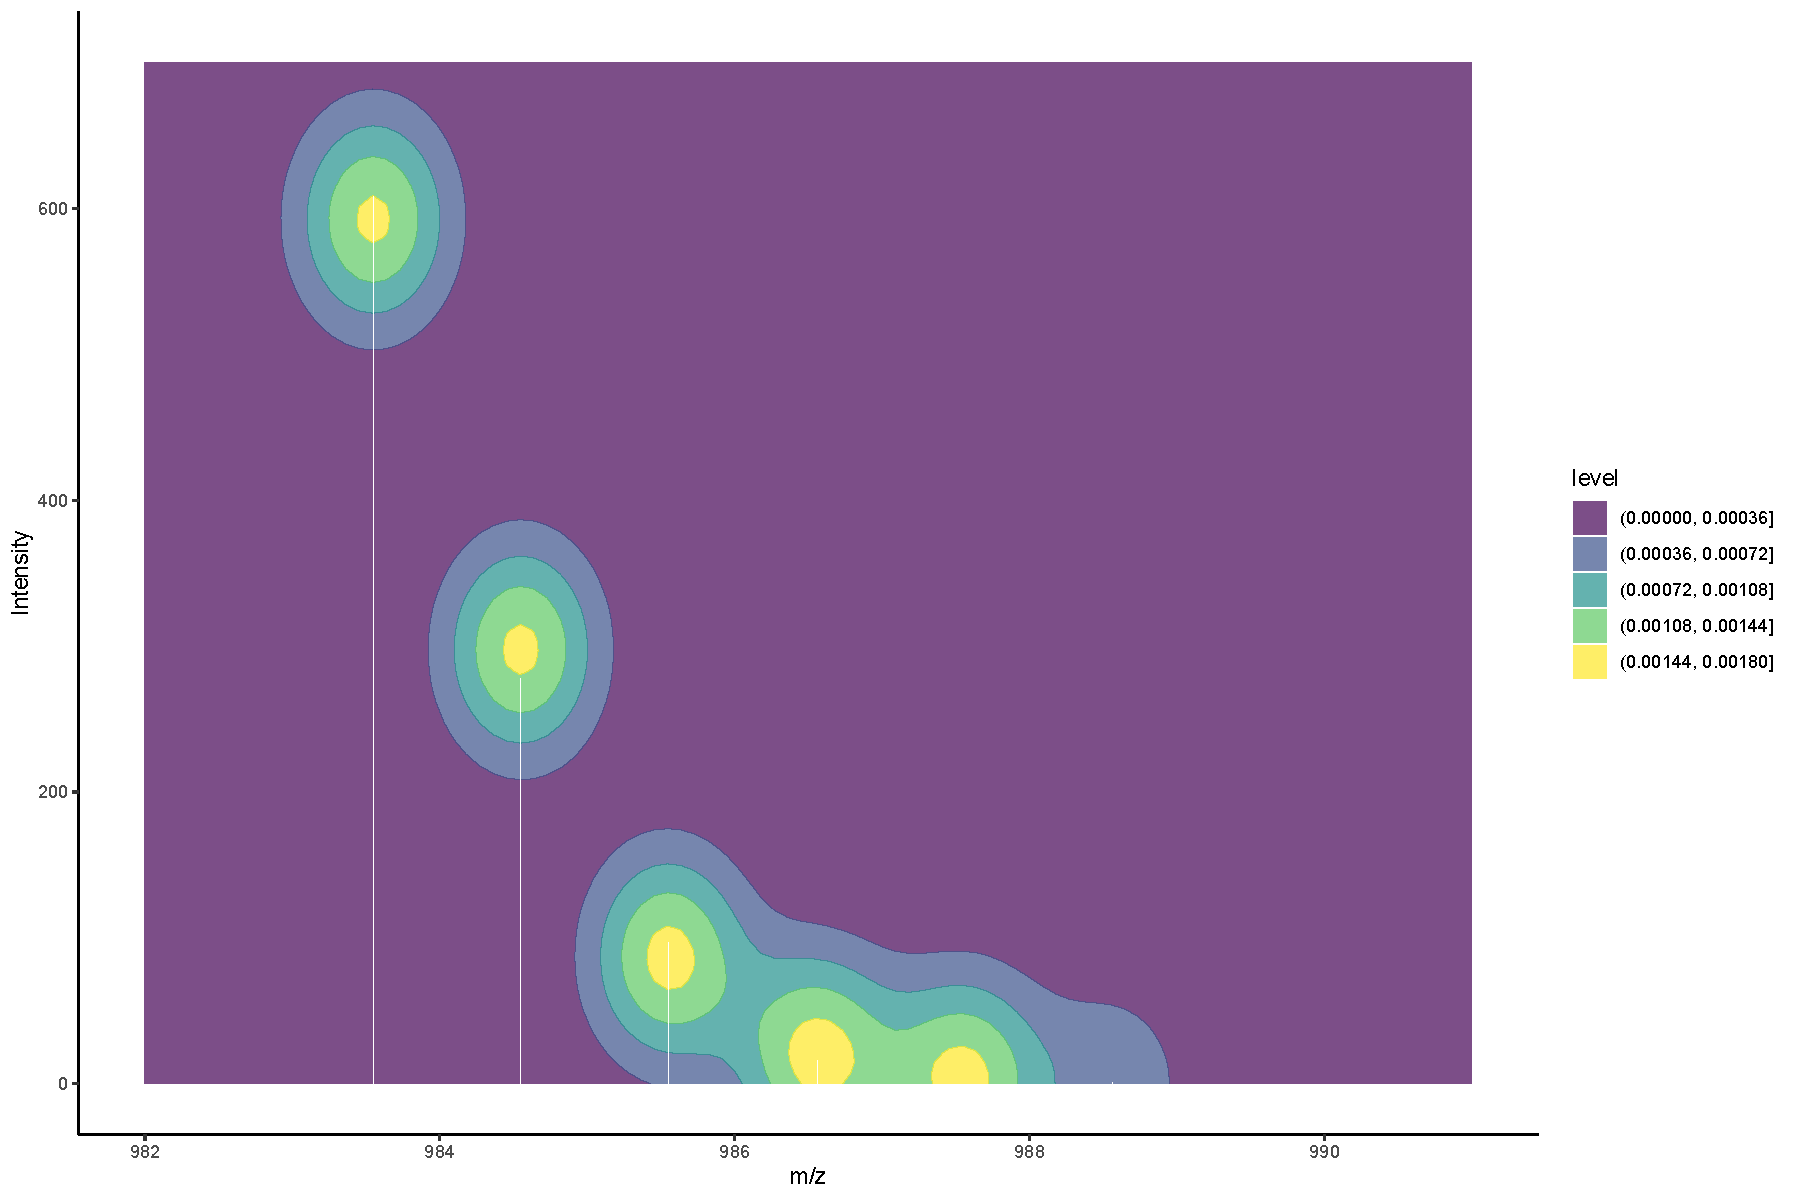
\includegraphics[width =1\textwidth]{spectrauncertaintyplot.pdf}
 	\caption{\textbf{Contour Spectra of PARRDAARA.} A contoured Spectra diagram showing the densities compatible with the MS1 spectra of PARRDAARA. Colour bar indicated relative probability. Example spectra overlaid in white.}
 	\label{figure::figure3spectrauncertaintyplot}
 \end{figure}

	
\end{document}